\documentclass[11pt,a4paper]{article}

\usepackage{titling}
\usepackage[hidelinks]{hyperref}
\usepackage{graphicx}
\usepackage{grffile}
\usepackage{float}
\usepackage{geometry}
\usepackage{listings}
\lstset{
	frame=single,
	breaklines=true,
}

\setlength{\parindent}{0pt}

\newcommand{\subtitle}[1]{
	\posttitle{
		\par\end{center}
	\begin{center}\large#1\end{center}
	\vskip0.5em}
}

\begin{document}
	\begin{figure}
		\centering
		
\includegraphics[height=150px]{../Images/CodusMaximus_logo.jpg}
	\end{figure}
	\begin{figure}
		\centering
		
\includegraphics[height=60px]{../Images/logo}
		\vspace{-50px}
	\end{figure}
	\title{ \textbf{User Manual}}
	\subtitle{ Organisation: \url{https://github.com/Hyperperform}}	
	\author{
		\textbf{Developers:} \\
		Rohan Chhipa		\emph{14188377}	\\
		Avinash Singh		\emph{14043778}	\\
		Jason Gordon		\emph{14405025}	\\
		Claudio Da Silva	\emph{14205892}	\\
	}
	
	\date{\textbf{Updated \today}}
	\maketitle
	\begin{center}
		\textbf{Client}
		\begin{figure}[H]
			\begin{center}
				
\includegraphics[width=0.20\columnwidth]{../Images/magna3}\\
				MagnaBC\\
				\url{http://www.magnabc.co.za/}
			\end{center}
		\end{figure}
	\end{center}
	
	\thispagestyle{empty}
	\pagebreak
	
	\tableofcontents
	\pagebreak

\section{System Overview}
Many different tools are available for measuring the quality of products made, but very few tools exist which assess the quality of the people making said products. People play a huge role in a project, and trying to monitor each and every one becomes a tedious task which diverts man power away from other more critical tasks. Whether it be for an end of year evaluation, or attempting to assess the current status of a project, generating a report on a staff member can help keep up productivity, as well as get them any help they need in order to resume quality performance. By ensuring that there is constant quality performance from each individual on a project, one can increase project quality as well as reduce project risks such as loss of an important team member during a critical stage of a project's life-cycle. \\ \\
The HyperPerform system has the ability to automatically gather information from multiple integrations such as GitHub and Travis. This alleviates the responsibility of the manager and HR having to manually monitor each employee by filling in time sheets and performance documents. The system aims to simplify management by allowing a manager to view all relevant employee data in a simple and easy to understand manner. This data is represented in the form of a report. These reports can be a summarised report or a more detailed report on an employees' activities. \\
In order to allow the system to be used in many different environments, we have developed the system to be highly pluggable in nature, so that one could easily increase the number of integrations from which information can be pulled.

\section{System Configuration}
This guide has been created for users who are using a Linux based operating system. To install the HyperPerform system on the machine you will be required to have an active connection to the internet. Please note that high amounts of data might be consumed during this process. 

\subsection{Docker installation}
To install the system with ease and to avoid all the system configurations you can download Docker to handle this for you. Docker can be found at \url{www.docker.com} where guides are made available for installing docker on a particular operating system. If you intend to use Docker to install the HyperPerform system then please ensure you install Docker on your machine.

\subsection{Manual Installation}
The manual installation requires you to download the source code from the GitHub repository. The newest release is highly recommended. To carry out a manual installation please ensure you have Maven and the WildFly application server on your machine. \\ \\
Maven can be downloaded from: \url{maven.apache.org} \\ \\
WildFly can be downloaded from: \url{wildfly.org} \\ \\
Please ensure you download WildFly 10. The HyperPerform system was fully tested on this version of WildFly. Any other version might produce unexpected behaviour. \\ \\
For the front-end Dashboard please ensure you have Nodejs (version 6.4.0 or higher) installed on your machine. Nodejs can be found at \url{https://nodejs.org/en/}.

\subsection{Event Gathering}
The system gathers information through webhook technology. Thus to be able to receive any events the computer on which the system will be installed \textbf{must} be connected to the internet. When configuring the integrations you will need to provide the URL for that integration to send events to. The following figure shows the GitHub webhook.

\begin{figure}[H]
	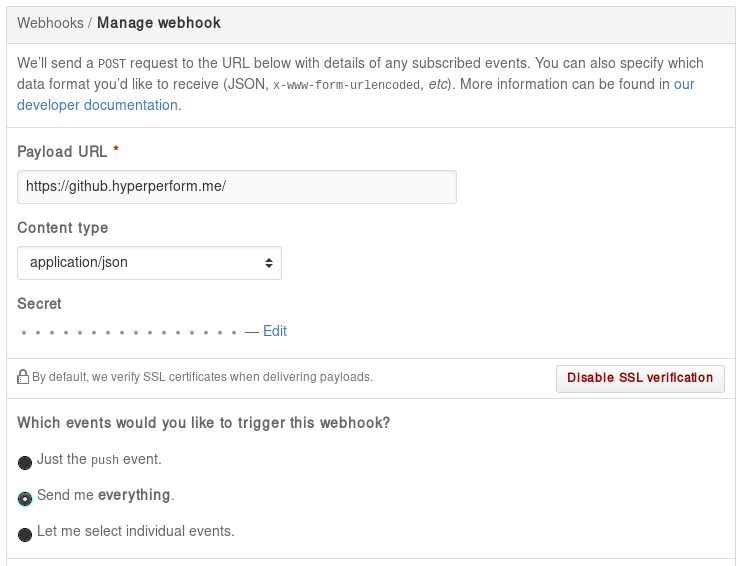
\includegraphics[width=\linewidth]{../Images/gitWebhook}
	\caption{Adding GitHub webhook}
\end{figure}

An optional feature would be to bind a domain name to the global IP address of the server. However this is merely for readability purposes and work affect system performance in any way.

\subsection{Miscellaneous}

Certain components of the system require user names which are consistent. The Git event processor is one such component. When using GitHub on your local machine please ensure that your local configurable Git name corresponds to your actual GitHub username. \\ \\
To check your local Git name open terminal or command prompt and run the following command: 

\begin{lstlisting}
git config user.name
\end{lstlisting} 
~\\
If the name corresponds to your account name then nothing further needs to be done and you can continue to the installation. However if the two names do not match then run the following command:

\begin{lstlisting}
git config --global user.name "<username>"
\end{lstlisting}
~\\
In the command above the $<$username$>$ is your actual account name.

\section{Installation}

\subsection{Docker Installation}

Assuming you have docker installed on your machine, simply run the following command in terminal: 

\begin{lstlisting}[language=bash]
docker run hyperperform/HyperPerform 
\end{lstlisting}
This will download the HyperPerform Docker image from DockerHub and run it on you machine. \\ \\
The front end component does not have a Docker image at this point in time. To install the front end component please refer to section 3.2.5 for the manual installation.

\subsection{Manual Installation}
This installation guide assumes a Linux Server running Ubuntu 14 or higher:

\subsubsection{WildFly}
Once you have downloaded the WildFly application server please carry out the WildFly installations and add a user. Once this is done proceed to installing PostgreSQL.

%Elevate to sudo permissions:

%\begin{lstlisting}
%sudo -s
%\end{lstlisting}
%Install Java JDK 8:
%\begin{lstlisting}
%aptitude update
%aptitude install --with-recommends software-properties-common
%add-apt-repository ppa:webupd8team/java
%aptitude update
%aptitude --with-recommends install oracle-java8-installer vim
%\end{lstlisting}
%Create a WildFly user:
%\begin{lstlisting}
%adduser --no-create-home --disabled-password --disabled-login wildfly
%\end{lstlisting}
%Download and extract the WildFly installation:
%\begin{lstlisting}
%cd /opt
%wget --tries=0 --continue http://download.jboss.org/wildfly/10.0.0.Final/wildfly-10.0.0.Final.tar.gz
%tar -xzvf wildfly-10.0.0.Final.tar.gz
%ln -s wildfly-10.0.0.Final wildfly
%chown -R wildfly wildfly
%\end{lstlisting}
%\pagebreak
%Copy the initialization scripts to the required folders:
%\begin{lstlisting}
%cp /opt/wildfly/docs/contrib/scripts/init.d/wildfly-init-debian.sh /etc/init.d/wildfly
%update-rc.d /etc/init.d/wildfly defaults
%cp /opt/wildfly/docs/contrib/scripts/init.d/wildfly.conf /etc/default/wildfly
%cd /etc/default
%\end{lstlisting}
%Now to edit the files:
%\begin{lstlisting}
%nano wildfly
%\end{lstlisting}
%Uncomment and/or Edit the following lines:
%\begin{lstlisting}
%JBOSS_HOME="/opt/wildfly"
%JBOSS_USER=wildfly
%JBOSS_MODE=standalone
%JBOSS_CONFIG=standalone-full.xml
%JBOSS_CONSOLE_LOG="/var/log/wildfly/console.log"
%\end{lstlisting}
%Change all 127.0.0.1 in standalone-full.xml to 0.0.0.0, then run the following commands:
%\begin{lstlisting}
%service wildfly start
%cd /opt/wildfly/bin
%./add-user.sh
%\end{lstlisting}

\subsubsection{PostgreSQL}
The install PostgreSQL on your machine: \\\\
Install via terminal:
\begin{lstlisting}
sudo apt-get update
sudo apt-get install postgresql postgresql-contrib
\end{lstlisting}
To configure PostgreSQL to connect remotely:
\begin{lstlisting}
sudo nano /etc/postgresql/9.3/main/postgresql.conf
\end{lstlisting}
Edit the following lines:
\begin{lstlisting}
listen_addresses = "*"
\end{lstlisting}
\pagebreak


\textbf{Create database hyperperform and the tables}\\
Run the following commands in terminal: 
\begin{lstlisting}
psql -c 'CREATE DATABASE hyperperform;' -U postgres

psql -d hyperperform -c 'CREATE TABLE public."GitPush" ( id integer NOT NULL, repository character varying(255), "timestamp" timestamp without time zone, username character varying(255), commitsize integer, url character varying(255), message character varying(255), CONSTRAINT "GitPush_pkey" PRIMARY KEY (id) ); CREATE SEQUENCE public.hibernate_sequence INCREMENT 1 MINVALUE 1 MAXVALUE 9223372036854775807 START 1 CACHE 1;' -U postgres

psql -d hyperperform -c 'CREATE TABLE public."TravisEvent" ( id integer NOT NULL, branch character varying(255), commiter character varying(255), repo character varying(255), status character varying(255), "timestamp" timestamp without time zone, CONSTRAINT "TravisEvent_pkey" PRIMARY KEY (id));' -U postgres

psql -d hyperperform -c 'CREATE TABLE public."CalendarProject" ( projectid integer NOT NULL, calendarid character varying(255), collaborators bytea, creator character varying(255), duedate timestamp without time zone, eventid character varying(255), reponame character varying(255), "timestamp" timestamp without time zone, CONSTRAINT "CalendarProject_pkey" PRIMARY KEY (projectid));' -U postgres

psql -d hyperperform -c 'CREATE TABLE public."CalendarMeeting" ( meetingid integer NOT NULL, calendarid character varying(255), creator character varying(255), duedate timestamp without time zone, eventid character varying(255), location character varying(255), "timestamp" timestamp without time zone, CONSTRAINT "CalendarMeeting_pkey" PRIMARY KEY (meetingid));' -U postgres

\end{lstlisting}
\pagebreak

\begin{lstlisting}
psql -d hyperperform -c 'CREATE TABLE public."CalendarMeeting_attendees" ( "CalendarMeeting_meetingID" integer NOT NULL, attendees integer, attendees_key character varying(255) NOT NULL, CONSTRAINT "CalendarMeeting_attendees_pkey" PRIMARY KEY ("CalendarMeeting_meetingID", attendees_key), CONSTRAINT fkn4q1pmj9vx3tfsaw9irp9voax FOREIGN KEY ("CalendarMeeting_meetingID") REFERENCES public."CalendarMeeting" (meetingid) MATCH SIMPLE ON UPDATE NO ACTION ON DELETE NO ACTION);' -U postgres

psql -d hyperperform -c 'CREATE TABLE public."GitIssue"(id integer NOT NULL, action character varying(255), assignee character varying(255), createdby character varying(255), issueid bigint, repository character varying(255), "timestamp" timestamp without time zone, title character varying(255), url character varying(255), CONSTRAINT "GitIssue_pkey" PRIMARY KEY (id));' -U postgres

psql -d hyperperform -c 'CREATE TABLE public."User" (email character varying(255) NOT NULL, gitusername character varying(255), name character varying(255), "position" integer, profilepicture bytea,  role integer, surname character varying(255), username character varying(255), password character varying(255), CONSTRAINT "User_pkey" PRIMARY KEY (email));' -U postgres

psql -d hyperperform -c 'CREATE TABLE "AccessEvent"(id integer NOT NULL, email character varying(255), day bigint, deviceid character varying(255), employeeid character varying(255), name character varying(255), surname character varying(255), "timestamp" timestamp without time zone, CONSTRAINT "AccessEvent_pkey" PRIMARY KEY (id) );' -U postgres

psql -d hyperperform -c 'CREATE TABLE public."ForecastData"(data character varying(10485760) NOT NULL, CONSTRAINT "ForecastData_pkey" PRIMARY KEY (data));' -U postgres


\end{lstlisting}

\pagebreak
\subsubsection{ActiveMQ}
To setup ActiveMQ on your server: \\
\begin{itemize}
	\item Start up your WildFly application server
	\item Navigate to WildFly management console on localhost:9990
	\item Navigate to configurations tab and click on sub-systems
	\item Scroll down and search for Messaging-ActiveMQ and click on it
	\item Click on default, select queues/topics
		\begin{figure}[H]
		\begin{center}
			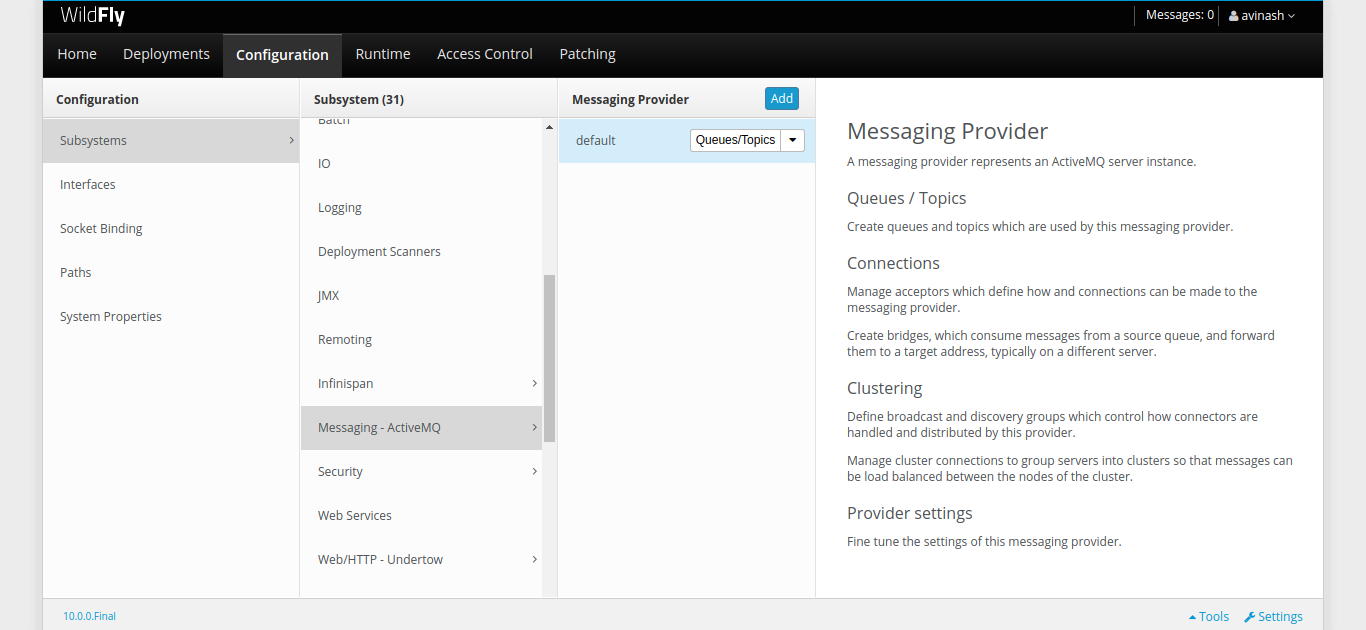
\includegraphics[width=\linewidth]{../Images/defaultqueue}
			\caption{Subsystems Configuration}
		\end{center}
	\end{figure}
	\item Click add and input the following information:
		\begin{itemize}
			\item Name*: hyperperform
			\item JNDI Names*: java:/jms/queue/hyperperform
		\end{itemize}
			\begin{figure}[H]
		\begin{center}
			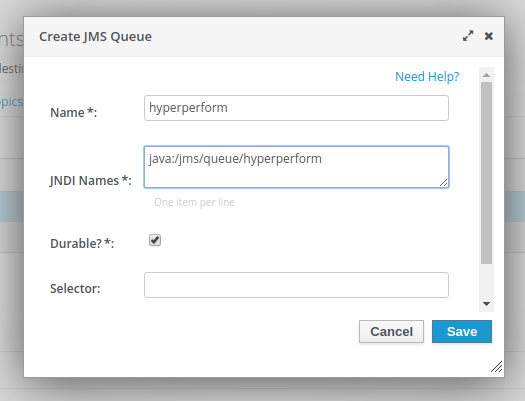
\includegraphics[scale=0.4]{../Images/queueconf}
			\caption{Queue Configuration}
		\end{center}
	\end{figure}
	
	\item Click save \\
\end{itemize}

\subsection{Notifications}
Please Note: These settings are for a Gmail configuration if you are running your own stmp server you need to adjust the information appropriately. 
To setup Notifications via Email on the server: \\
\begin{itemize}
	\item Start up your WildFly application server
	\item Navigate to WildFly management console on localhost:9990
	\item Navigate to configurations tab and click on sub-systems
	\item Scroll down and search for Email and click on it
	\begin{figure}[H]
		\begin{center}
			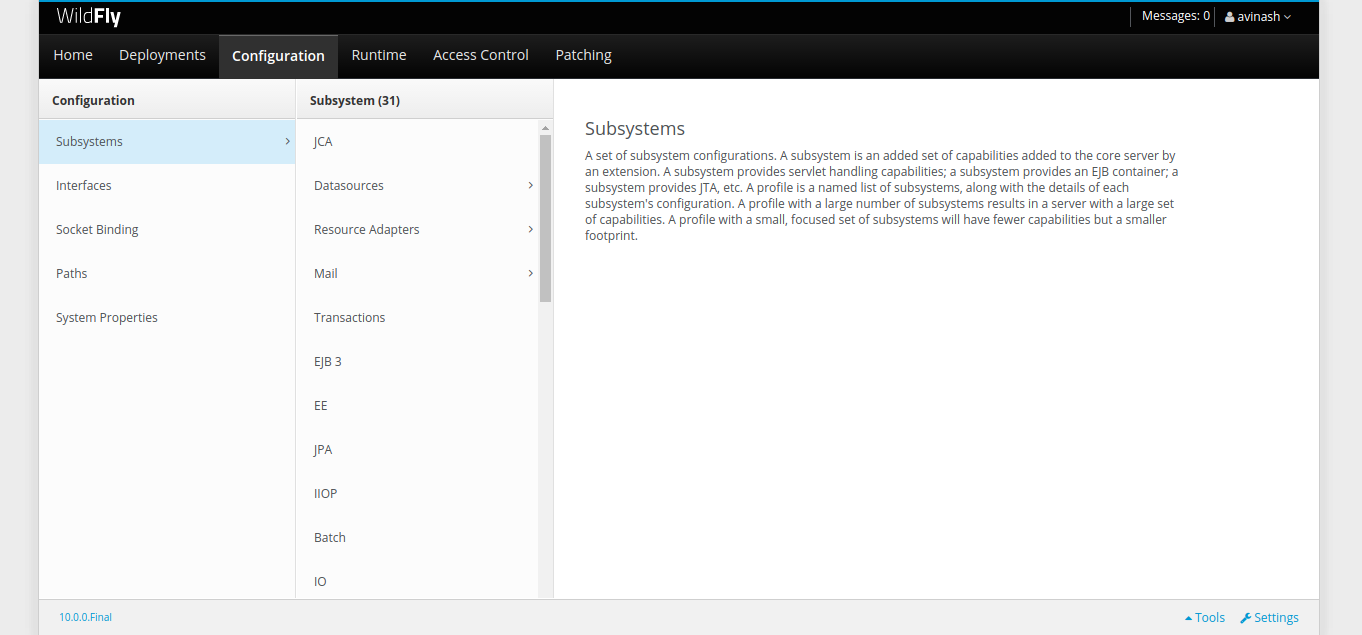
\includegraphics[width=0.6\linewidth]{../Images/subsystem}
			\caption{Subsystem Email}
		\end{center}
	\end{figure}
	\item Click add and input the following information:
	\begin{itemize}
		\item Name*: Gmail 
		\item JNDI: java:/jboss/mail/gmail
	\end{itemize}
	\item Click save \\
	\item There after View the new configuration and Add a new type
	\begin{itemize}
		\item Socket-binding: mail-smtp
		\item Type: smtp
		\item Username: "Your@gmail account"
		\item Password: "Gmail password"
		\item SSL: enable
	\end{itemize}
	\item There after reload the server
	\item After reloading navigate to configurations tab and the Socket Bindings
		\begin{figure}[H]
		\begin{center}
			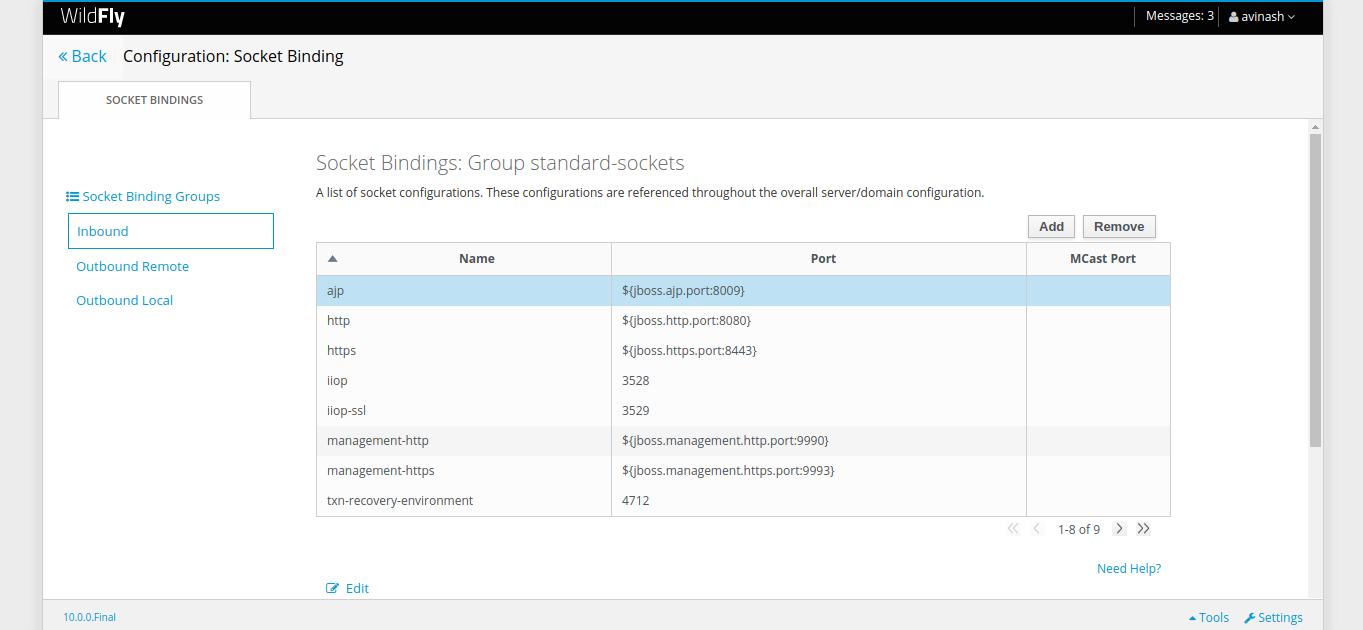
\includegraphics[width=\linewidth]{../Images/socket}
			\caption{Socket Bindings}
		\end{center}
	\end{figure}
	\item Click on View and there after under standard-sockets click view
	\item Navigate to Outbound Remote and edit the mail-smtp socket bindings
		\begin{itemize}
		\item Host: smpt.gmail.com
		\item Port: 465
	\end{itemize}
	\begin{figure}[H]
	\begin{center}
		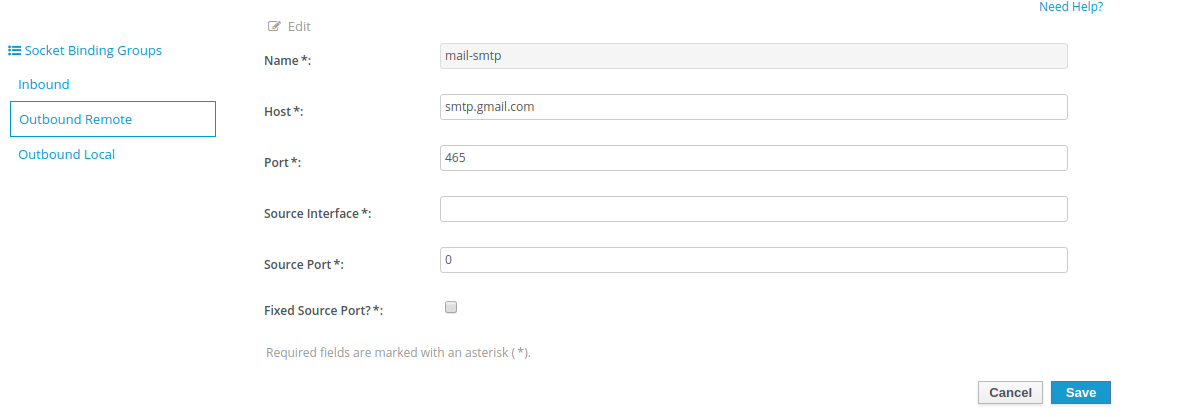
\includegraphics[width=\linewidth]{../Images/outbound}
		\caption{Outbound Socket Configuration}
	\end{center}
\end{figure}
	\item Reload server
\end{itemize}


\subsubsection{Deploying to WildFly}
To deploy the HyperPerform system to the application you will need to build the system using from the source code. 

\begin{itemize}
	\item Ensure the WildFly server is running.
	\item Navigate to \url{https://github.com/HyperPerform/hyper-perform-server/releases} and download the newest release source code.
	\item Extract the source code
	\item Navigate to the root directory of the source code. A file named pom.xml should be clearly visible.
	\item Run the following command: mvn clean wildfly:deploy
	\item Maven will then ask you to provide your user name and password for the Wildfly Server.
	\item Thereafter Maven will automatically deploy the compiled code (war) to WildFly
\end{itemize}



\subsubsection{Front-end Dashboard}
Please notee that there is no release yet for the dashboard and there might be a few bugs, or limitations to the software.\\
To start up the front end please ensure you have Node 6.4.0 or higher installed on your machine. Node can be found at \url{https://nodejs.org/en/}. \\\\\\
\noindent
\textbf{Please make sure that these commands execute successfully before attempting to run the system:}
\begin{lstlisting}
	 npm install -g gulp
	 npm install -g bower
	 npm install -g sass
\end{lstlisting}
Once that has completed with no errors do the following.
\begin{itemize}
	\item Download the Dashboard source code from \url{https://github.com/HyperPerform/hyper-perform-web-application}
	\item Navigate to the root directory of the source code
\end{itemize}
Run the following commands in terminal: 
\begin{lstlisting}	
	npm install
	gulp build
	gulp serve
\end{lstlisting}
\noindent
The front-end system will auto launch in your default browser in order to view the data in the front-end system the Wildfly application server must be running.

%\pagebreak

%\section{Installation of HyperPerform}
%
%\subsection{Server}
%To setup the back end, take the hyperperform.war and deploy it on the WildFly management console
%
%\subsection{Dashboard}
%To install the dashboard on your server:
%\begin{lstlisting}
%npm install hyperperform
%\end{lstlisting}
\pagebreak
\section{Getting Started/Using the System}
Once the front-end Dashboard is served your default browser should automatically open. In the event that it didn't, simply open the browser of your choice and navigate to the following URL: \url{localhost:3000}. 

\subsection{Logging In}
Once the Dashboard loads you will be presented with the following screen:

\begin{figure}[H]
	\begin{center}
		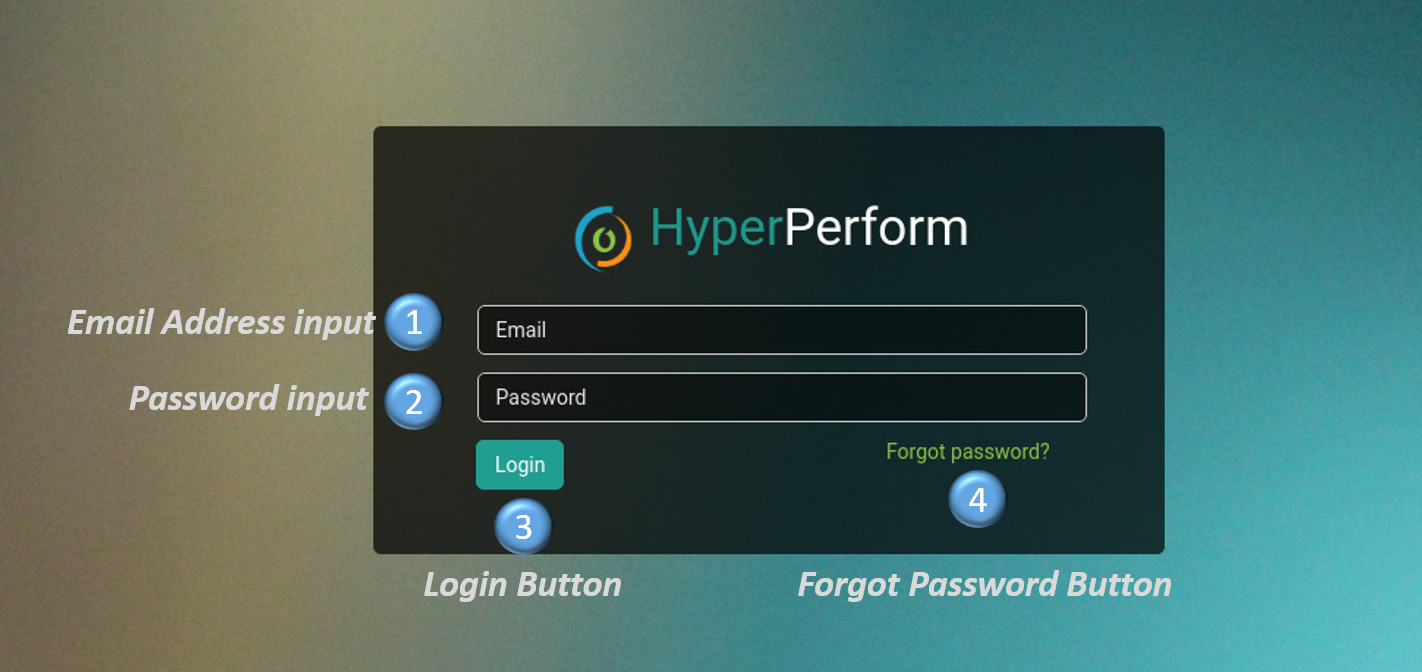
\includegraphics[scale=0.3]{../Images/Getting_Started/Login_numbered}
		\caption{Login screen}
	\end{center}
\end{figure}
\noindent
The default username and password is Admin. This is a default login for when the system is installed for the first time. Once managers exist within the database this feature will be disabled for security purposes.

\subsection{Your Dashboard}
Once logged in the user will be presented with the following screen:

\begin{figure}[H]
	\begin{center}
		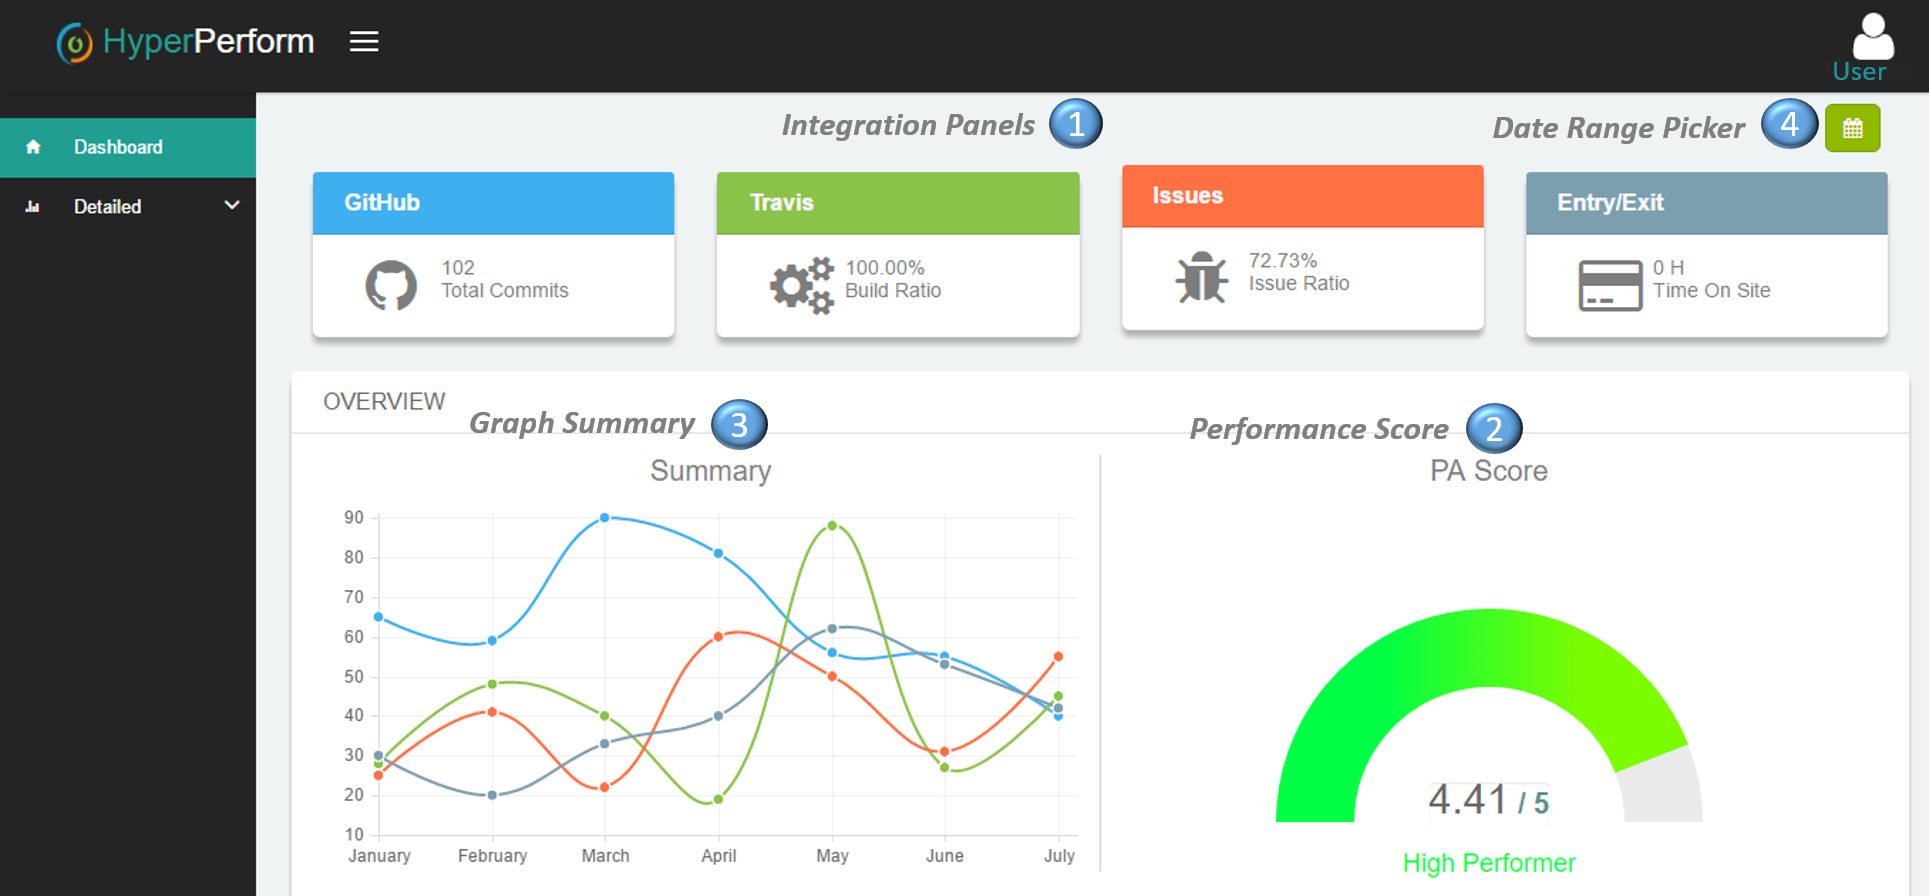
\includegraphics[scale=0.27]{../Images/Getting_Started/dash_numbered.png}
		\caption{Dashboard}
	\end{center}
\end{figure}
\noindent
On this screen you are given a summarised view of all the integrations parts of the HyperPerform system. Note the four colour-coded panels on top, each of these panels represents an integration. These panels are click-able and will direct you to a details screen which will be discussed in the next section 5.

\subsubsection{Filtering Your Performance Score}
\begin{figure}[H]
	\begin{center}
		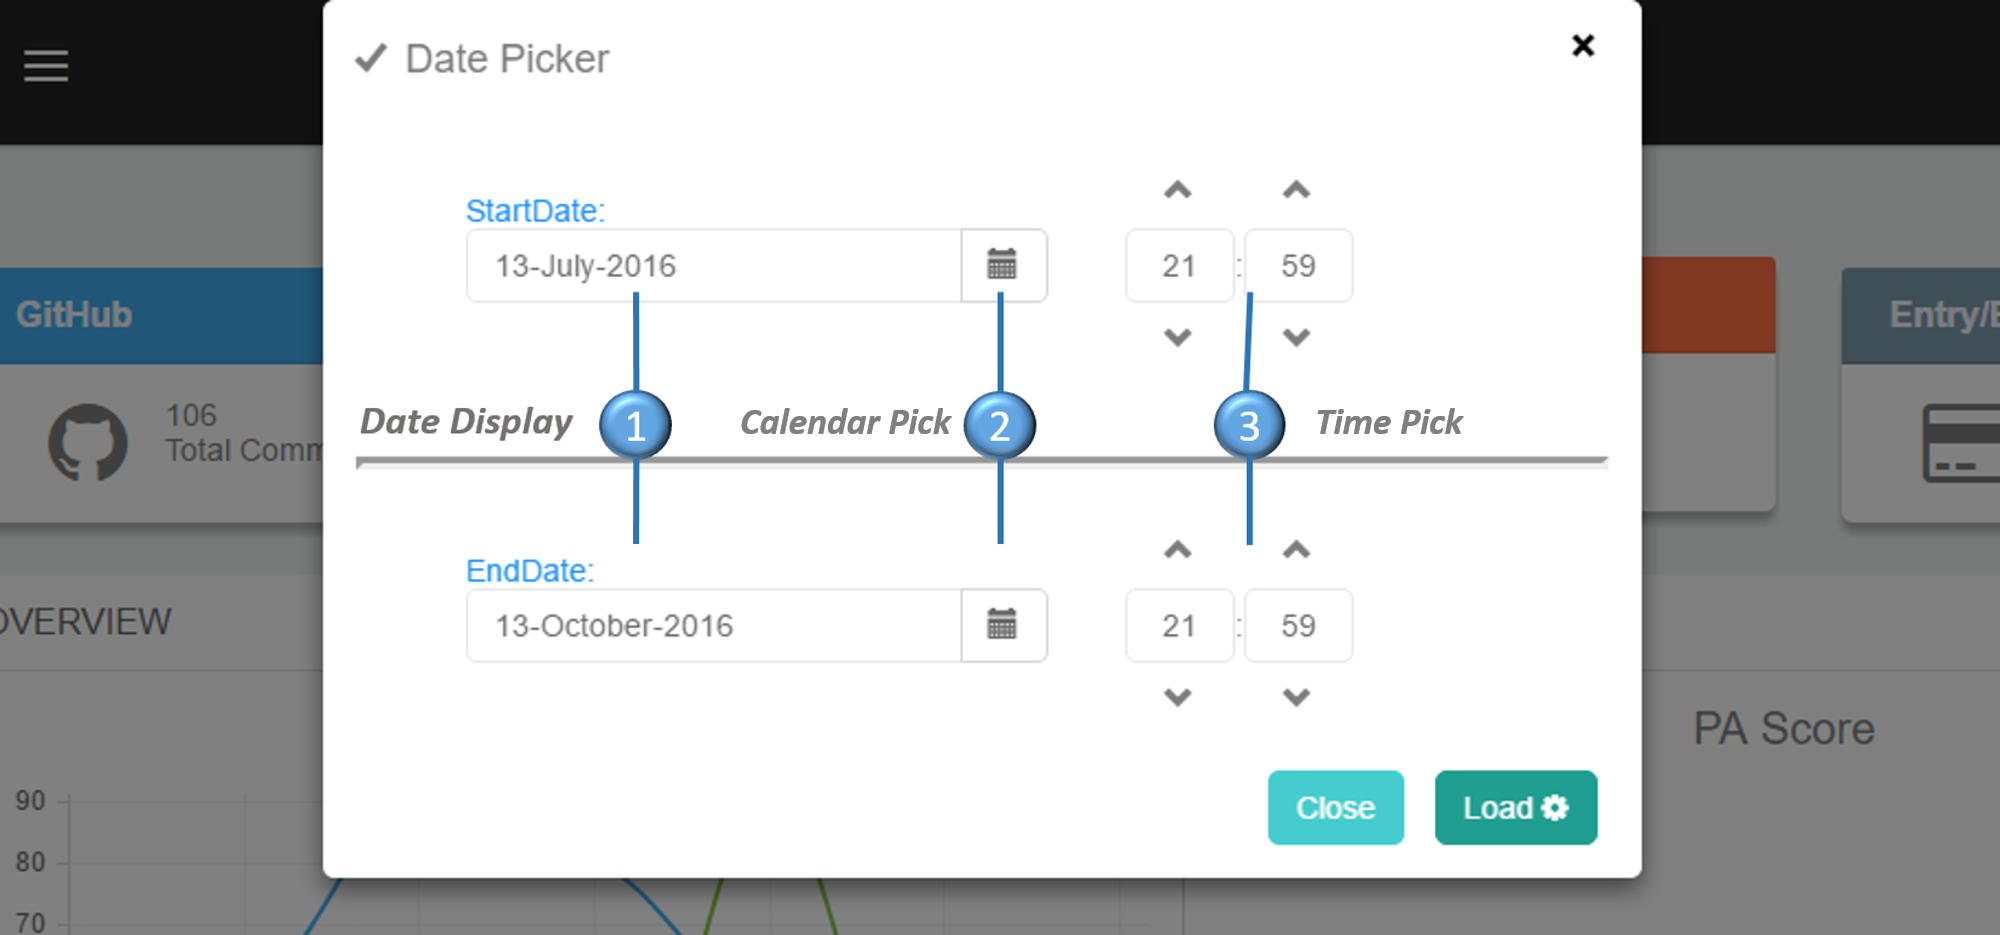
\includegraphics[scale=0.27]{../Images/Getting_Started/Date_Picker_Numbered}
		\caption{Date Picker}
	\end{center}
\end{figure}
\noindent

\subsection{Detailed View}
\subsubsection{Graph View}
\begin{figure}[H]
	\begin{center}
		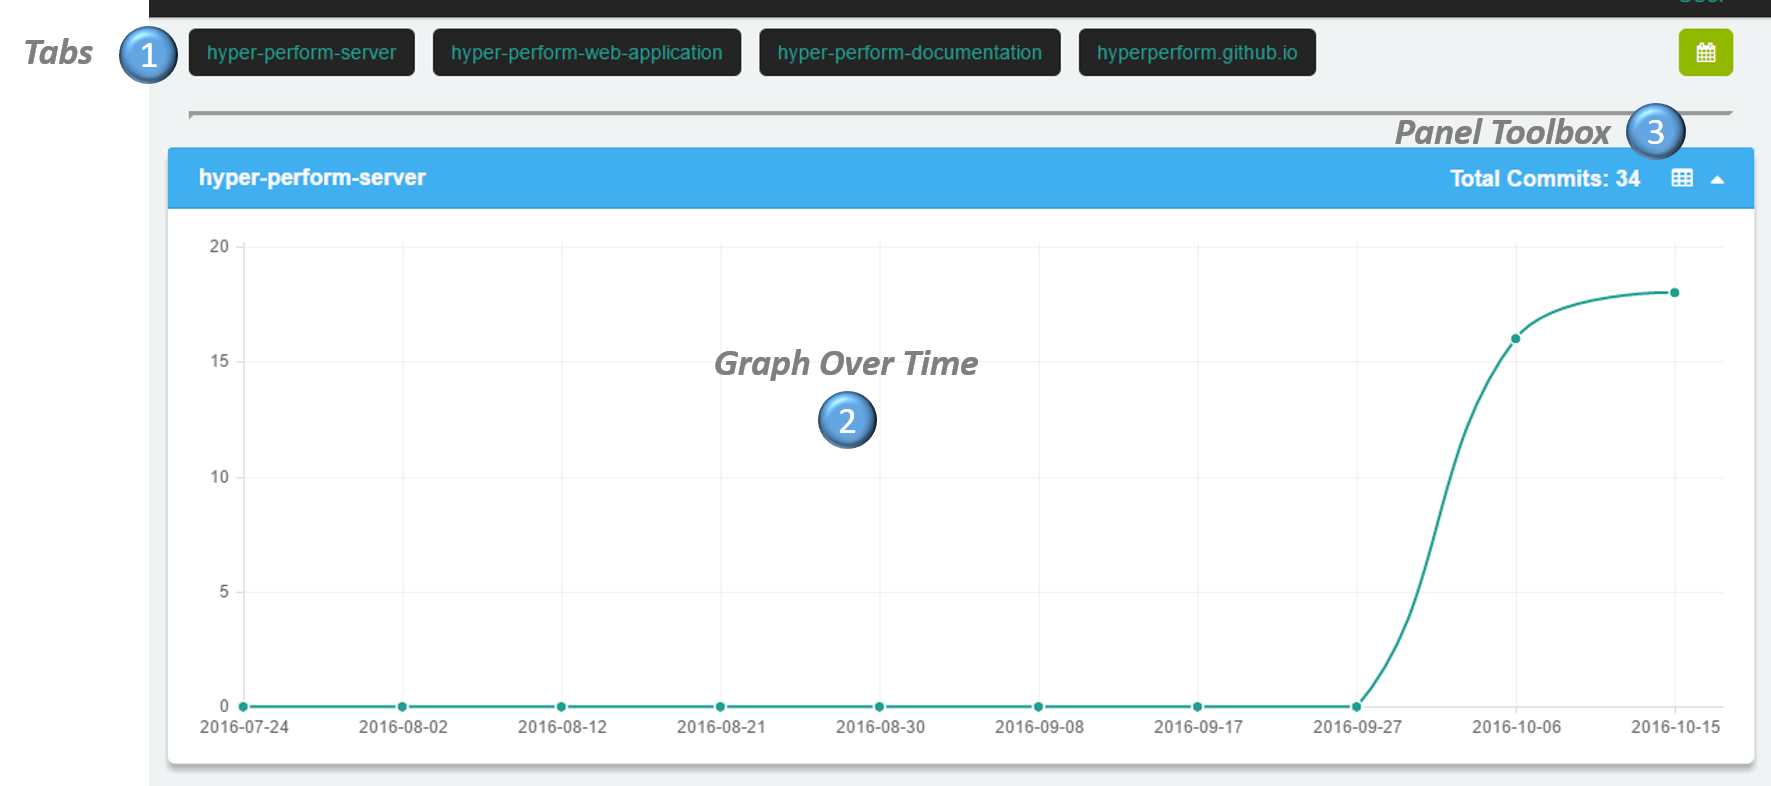
\includegraphics[scale=0.27]{../Images/Getting_Started/GitHub_Detailed_Graph_numbered}
		\caption{Detailed View Graph}
	\end{center}
\end{figure}

\subsubsection{Table View}
\begin{figure}[H]
	\begin{center}
		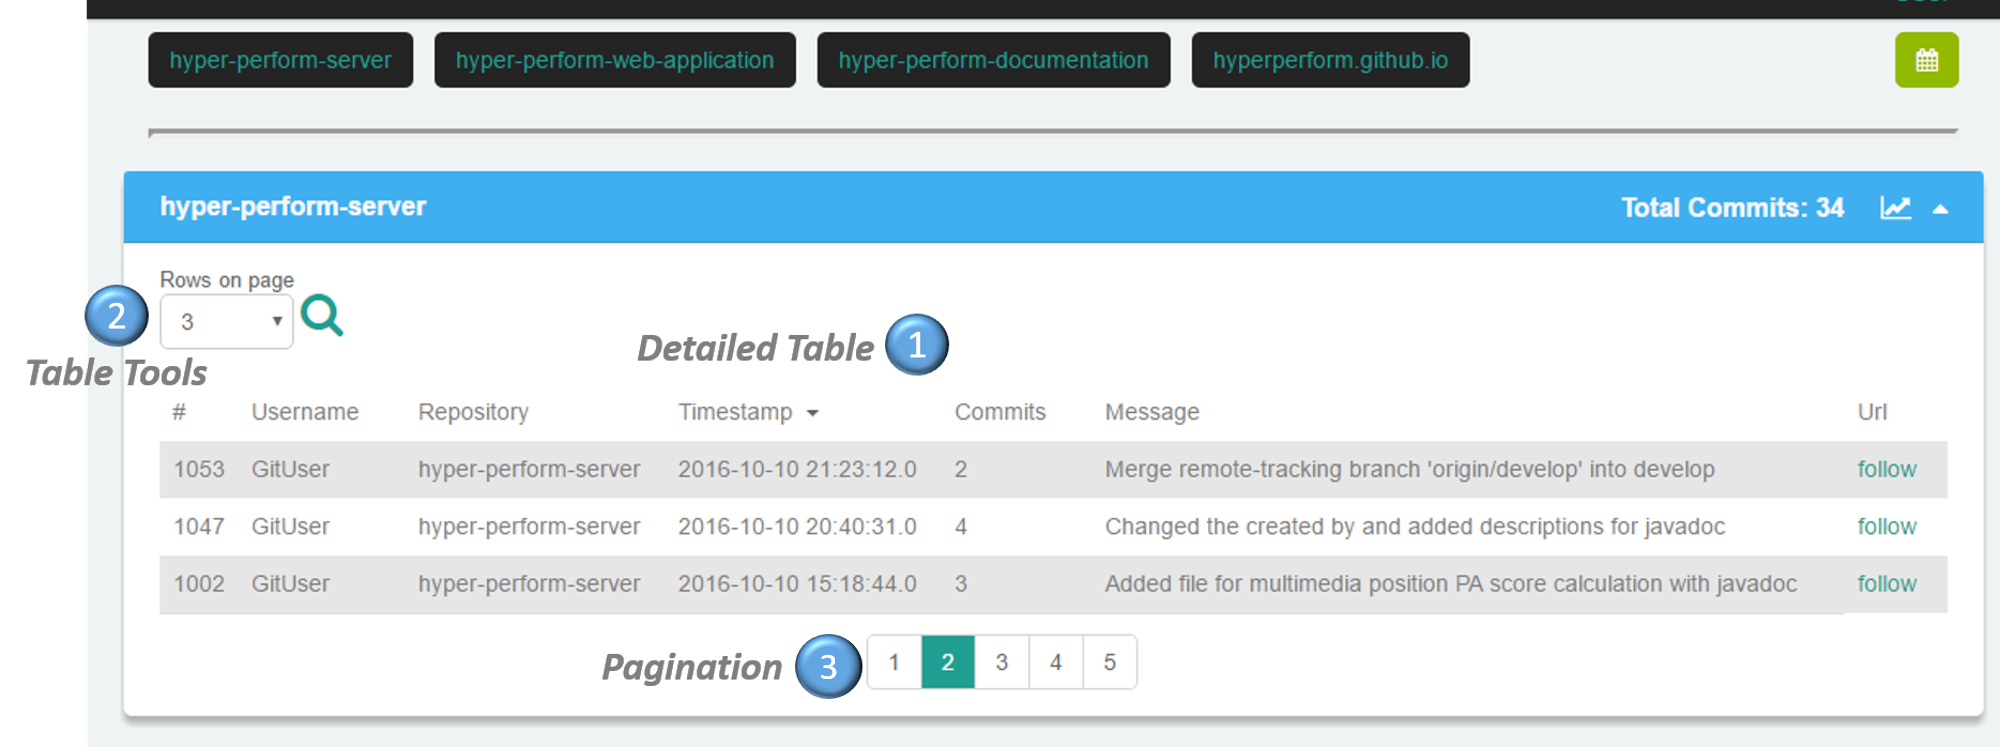
\includegraphics[scale=0.27]{../Images/Getting_Started/GitHub_Detailed_Table_numbered}
		\caption{Detailed View Graph}
	\end{center}
\end{figure}

\subsection{Signing Out}
If you wish to logout then you merely click on the profile icon in the top right corner. Once clicked you will be presented with a small menu. 

\begin{figure}[H]
	\begin{center}
		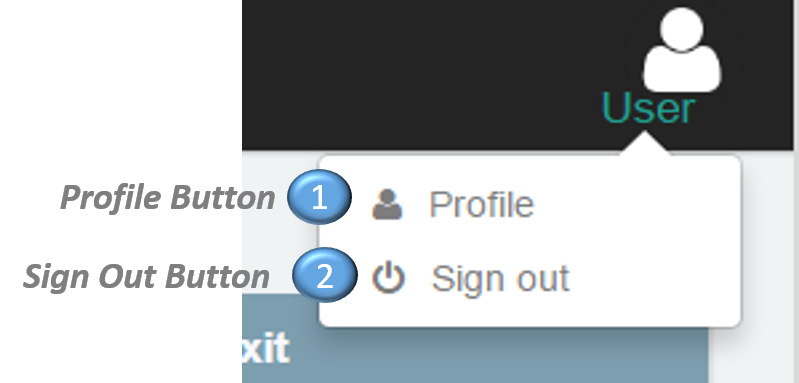
\includegraphics[scale=0.7]{../Images/Getting_Started/logout_numbered}
		\caption{Signing Out}
	\end{center}
\end{figure}

\begin{enumerate}
	\item \textbf{Sign Out Button:}
		\begin{enumerate}
			\item For an employee - When this button is pressed it will sign you out of your dashboard and you will be redirected back to the login page (Figure 7).
			\item For a manager - This button will sign you out of your employees' dashboard and redirect you to the Employee List Page (Figure ?) where you can view other employees' performance.
		\end{enumerate} 
\end{enumerate}
\noindent
In this menu you have a few options to choose from. The Profile option will direct you to a profile page where you will be able to view and edit your current details. \\ \\
The second option is a simple settings page where you can customize the dashboard.\\ \\
And finally the Sign Out option can be used to log off the system. Once logged off you will be returned to the login screen in Figure 1.

\pagebreak

\section{Managerial features}
A variety of features are only made available to the manager within the organisation.

\subsection{Managerial view}
When a manager logs into the system, instead of being directed to a dashboard they will be directed to the following view.

\begin{figure}[H]
	\begin{center}
		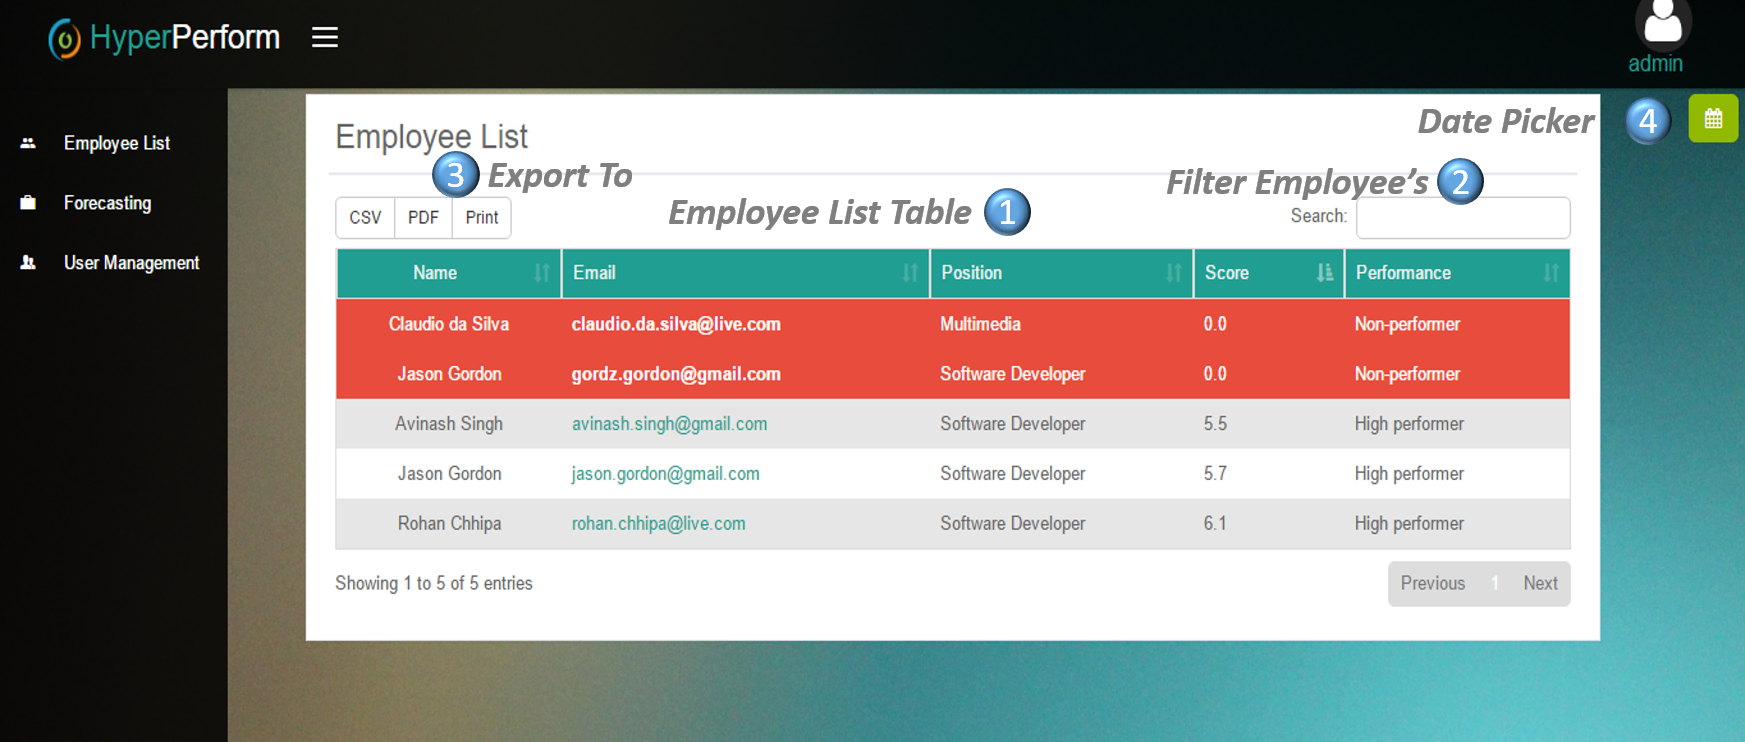
\includegraphics[width=\linewidth]{../Images/Getting_Started/Man_page_numbered}
		\caption{Managerial view}
	\end{center}
\end{figure}

\noindent
From this screen a manager is able to view all the current employees within the organisation. They can see all the necessary employee data such as name, email, performance score and performance classification. \\ \\ 
\noindent
A manager also has the ability to view an employees' dashboard. This can be achieved by simply clicking on the employees' name and the manager will be directed to the corresponding employees' dashboard. \\ \\
\noindent
Managers also have the ability to export the table to a PDF or CSV file or even directly print it out. This allows the manager to keep a copy with them at any time and can aid with record keeping by allowing them to print the table at regular intervals.

\subsection{User registration}
The responsibility of adding users to the system is given to the manager. When registering a new user the manager must go through a three step registration process.

\begin{figure}[H]
	\begin{center}
		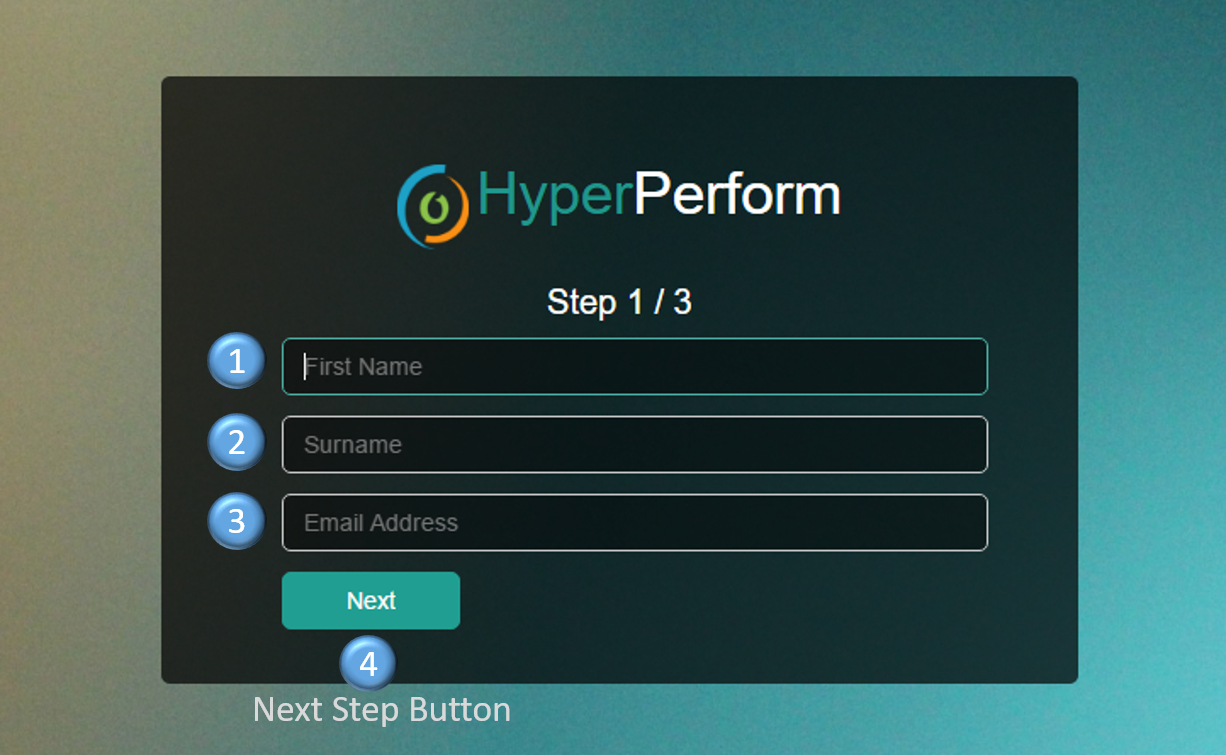
\includegraphics[scale=0.35]{../Images/Getting_Started/Step_1_numbered}
		\caption{Registration step 1}
	\end{center}
\end{figure}

\noindent
In this step the manager needs to enter basic information such as employee firstname, surname and email address. 

\begin{figure}[H]
	\begin{center}
		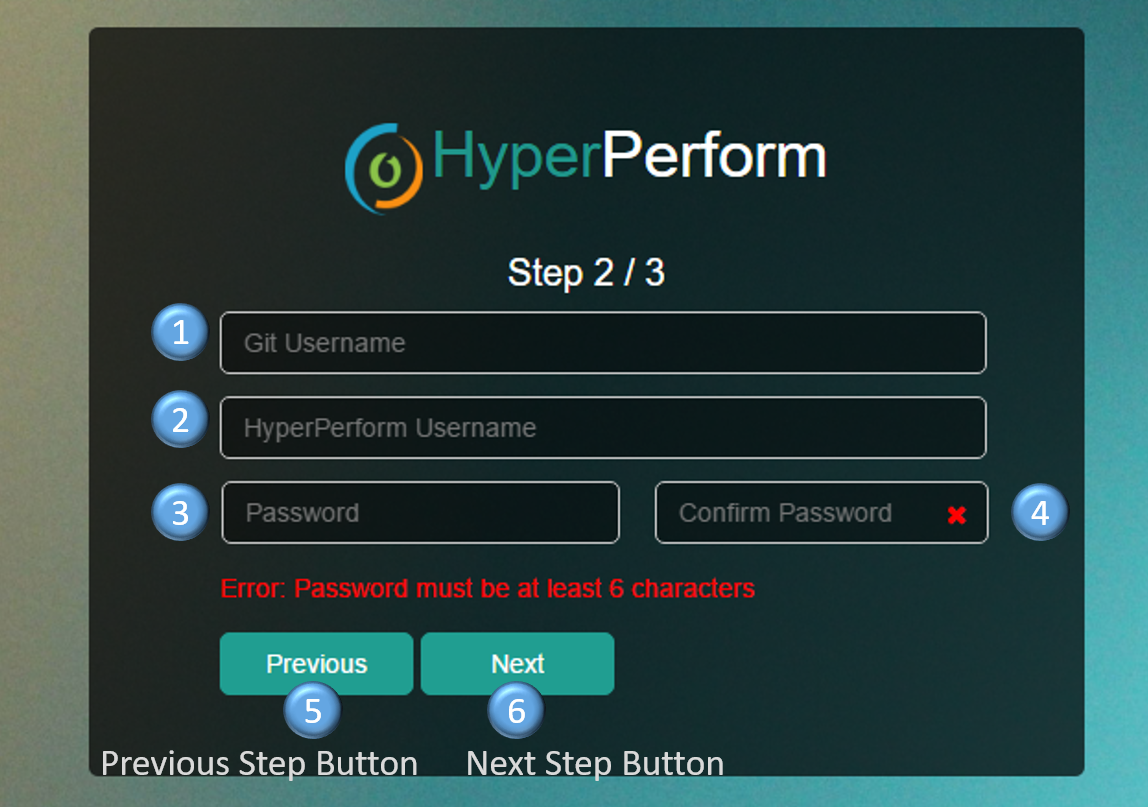
\includegraphics[scale=0.35]{../Images/Getting_Started/Step_2_numbered}
		\caption{Registration step 2}
	\end{center}
\end{figure}

\noindent
This step requires the employees' GitHub username. This is very important when processing that employees' GitHub data. The manager can give the employee a HyperPerform system username and a password.

\begin{figure}[H]
	\begin{center}
		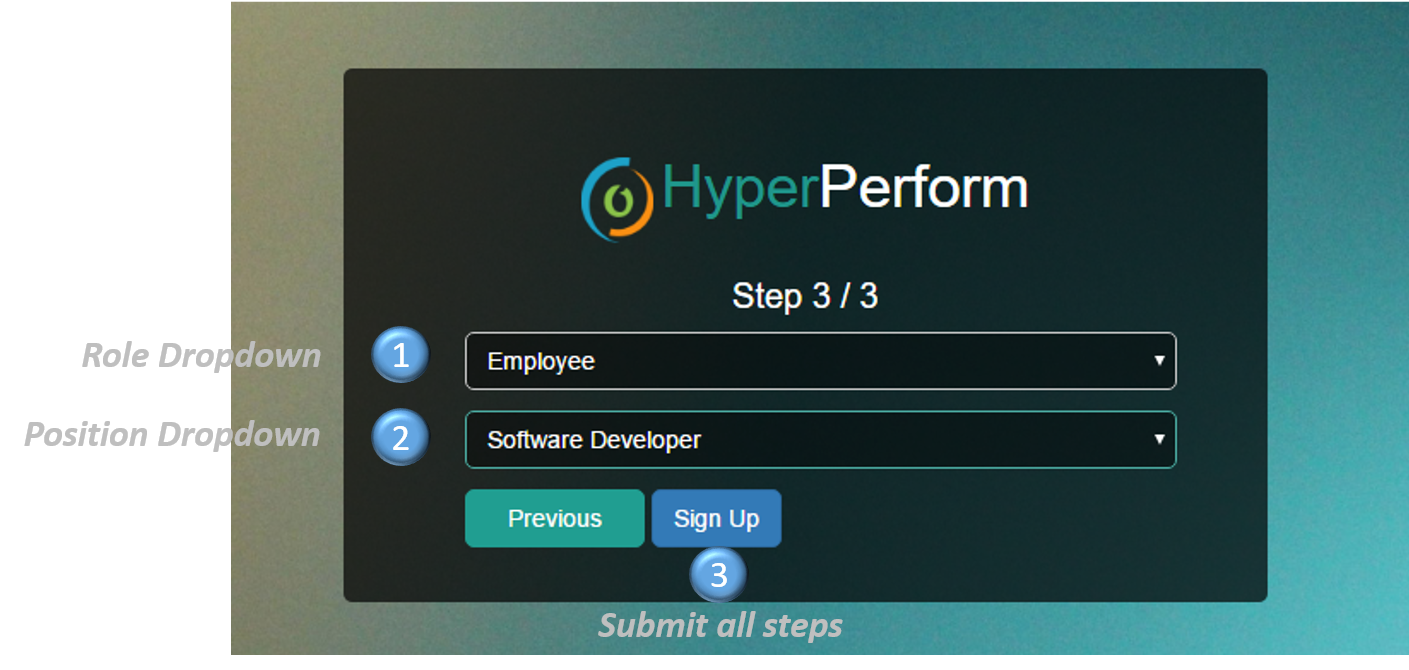
\includegraphics[width=\linewidth]{../Images/Getting_Started/Step_3_numbered}
		\caption{Registration step 3}
	\end{center}
\end{figure}

\noindent
In the final step the manager must specify the employees' role and position within the organisation. \\ \\
\noindent
Currently existing roles are:
\begin{itemize}
	\item Administrator
	\item Employee \\
\end{itemize}
\noindent
Currently existing positions are:
\begin{itemize}
	\item Web Developer
	\item Software Developer
	\item Multimedia
\end{itemize}

\pagebreak

\subsection{Forecasting}
The forecasting section allows for an administrator to add forecast values to the system. A forecast value is a prediction made by an administrator with regards to employee performance.
\begin{figure}[H]
	\begin{center}
		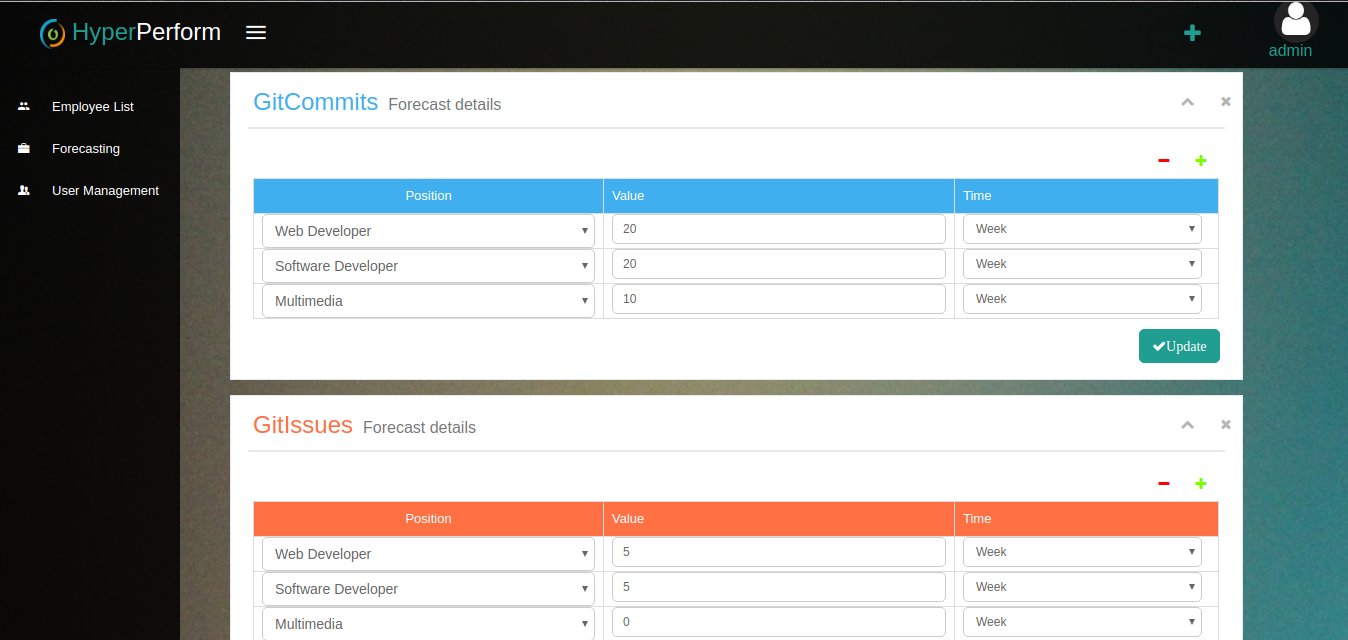
\includegraphics[width=\linewidth]{../Images/Getting_Started/forecast}
		\caption{Dashboard errors}
	\end{center}
\end{figure}

An administrator can add a forecast for each integration and assign it to a particular employee position. Thus different employee positions may have different forecast values for the same integration. \\

Each integration is displayed to the administrator on the forecasting page. Each integration is displayed in its own panel. Each panel consists of a table which shows each position along with its corresponding forecast value. \\

The tables can be directly changed. Once all the changes are made simply click on the tables update button to send the changes off to the server. If the administrator does not wish to directly modify the table then simply click on that particular tables + button. This will allow the administrator to add a new row to the table. \\

New integrations can also easily be added. Simply click on the + on the navbar to bring up a modal(Figure ?). On this modal a new integration can be added to the system. \textbf{Note:} when adding a new integration, at least one position and forecast value must be added. 

\section{Errors}
\begin{figure}[H]
	\begin{center}
		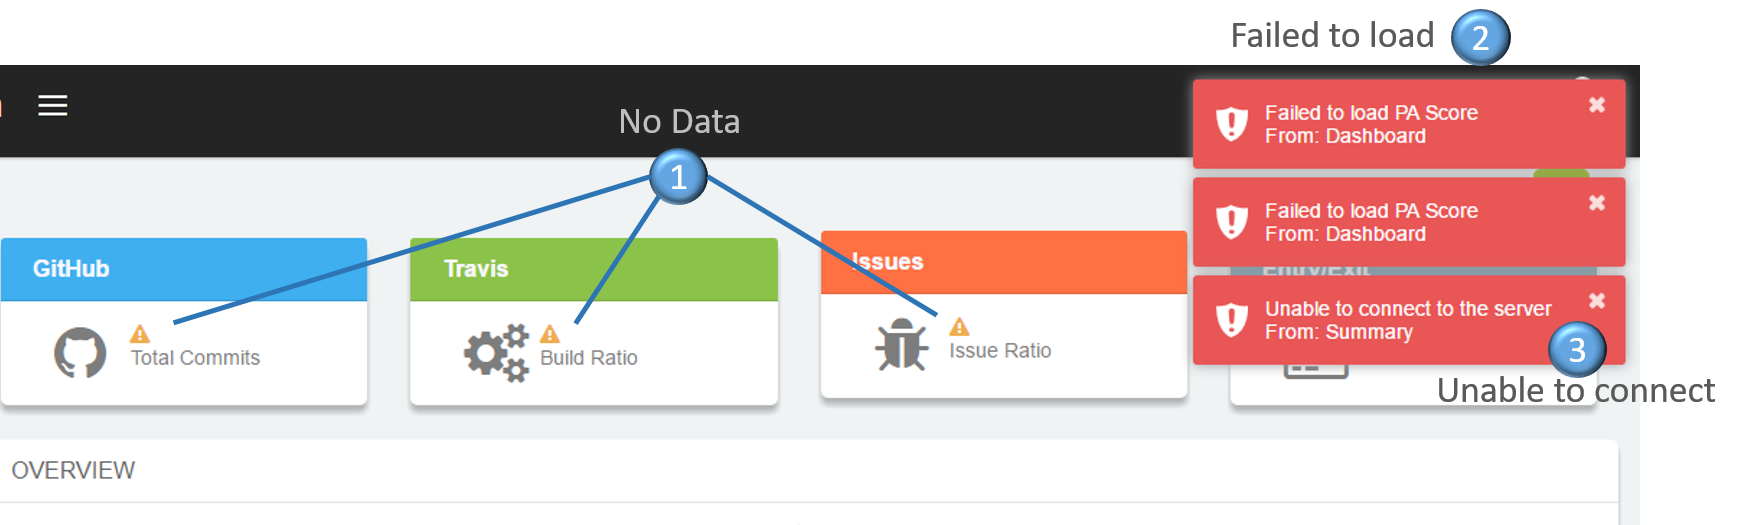
\includegraphics[width=\linewidth]{../Images/Getting_Started/Dash_Error_numbered}
		\caption{Dashboard errors}
	\end{center}
\end{figure}

\begin{figure}[H]
	\begin{center}
		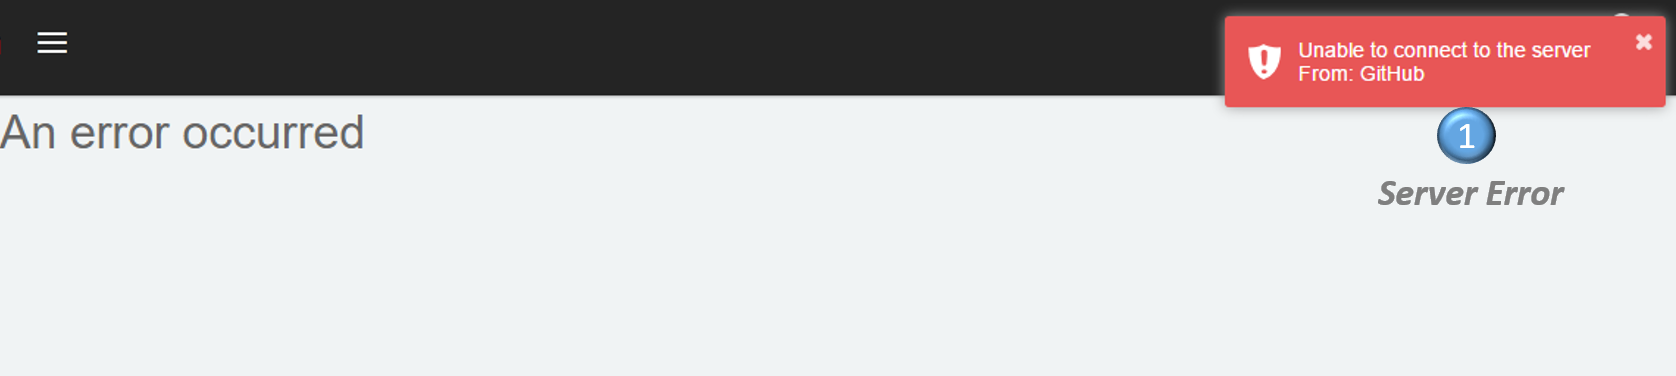
\includegraphics[width=\linewidth]{../Images/Getting_Started/Connect_Server_Detailed_numbered}
		\caption{Server connection error}
	\end{center}
\end{figure}

\begin{figure}[H]
	\begin{center}
		
\includegraphics[width=\linewidth]{../Images/Getting_Started/No_Data_Detailed_numbered}
		\caption{No data error}
	\end{center}
\end{figure}

\end{document}